\documentclass{article}
\usepackage[utf8]{inputenc}
\usepackage{amstext}
\usepackage{amsmath} 
\usepackage{mathpazo}
\usepackage{graphicx} 
\usepackage{float} 
\usepackage{caption} 
\usepackage{epstopdf} 
\usepackage{hyperref}
\usepackage{varioref} 
\usepackage{fancyref}
\usepackage[section]{placeins} 
\usepackage{perpage}
\usepackage[margin=1in, paperwidth=8.5in, paperheight=11in]{geometry} 
\MakeSorted{figure} 
\usepackage{natbib}
\usepackage{graphicx}
\usepackage{xcolor}
\usepackage{listings}
\usepackage{minted}
\usepackage{subcaption}
\usepackage{eso-pic}
\usepackage{tikz}
\usepackage[american]{circuitikz}
\usepackage[font=small,labelfont=bf]{caption}

\title{ENGR2420 Lab 3 : Resistors and Bipolar Transistors}
\author{Abigail Fry \\ Anusha Datar \\ Vienna Scheyer}
\date{February 23, 2019}

\begin{document}

\maketitle

\section{Experiment One: Forward Active Bipolar Transistor Characteristics}
In this experiment, we used the Source Measurement Unit to measure the the base and emitter current  of a 2N3904 bipolar transistor using the schematic in Figure \ref{fig:exp1_sch}.  We recorded the base and emitter current values while sweeping input voltages from .25 Volts to .75 Volts, which yielded current values from approximately 10 nA to 20 mA.  Using the base and emitter current measurements, we were able to calculate the collector current for the experimental voltage range.
\begin{figure}[H]   
  \centering        
  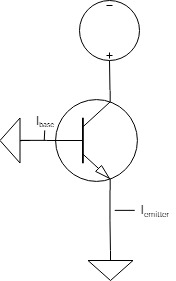
\includegraphics[scale = 0.5]{images/experiment_one_schematic.jpg}
  \caption{The schematic for the circuit used to determine the current-voltage characteristic of the transistor.}   
  \label{fig:exp1_sch}
\end{figure}

\subsection{Results}
We calculated the collector current by finding the difference between the base current and the emitter current of the transistor as we swept through a selected range of voltages. 

The plot in Figure \ref{fig:exp1_vc} shows the current-voltage characteristic of the input voltage at the base of the transistor and the base and collector current responses. 
\begin{figure}[H]   
  \centering        
  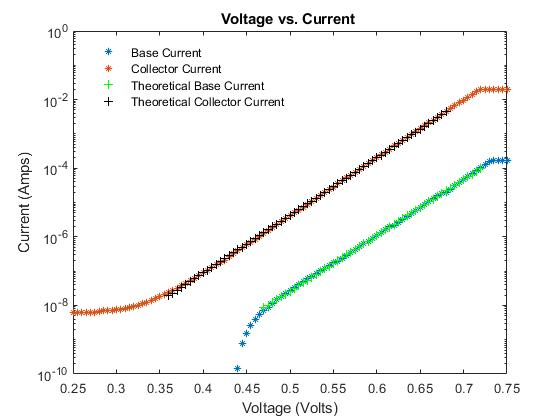
\includegraphics[scale = 0.5]{images/pt1_exp1.jpg}
  \caption{The current-voltage characteristic of the transistor at the base and collector.}   
  \label{fig:exp1_vc}
\end{figure}

From the slope of the current-voltage characteristic, we were able to  quantify the resistive behavior of the transistor. The current-voltage response's slope is 37.46 $\Omega$ at the base and 38.59 $\Omega$ at the collector. We also used linear regression to determine that the experimental value of the thermal voltage, $U_T$, was 0.026 Volts.

The plot in Figure \ref{fig:exp1_beta} shows the collector current plotted against the current gain $\beta$ where $\beta$ is the ratio of the partial derivative of the collector current to the partial derivative of base current, $\frac{\partial I_{c}}{\partial I_{b}}$.

\begin{figure}[H]   
  \centering        
  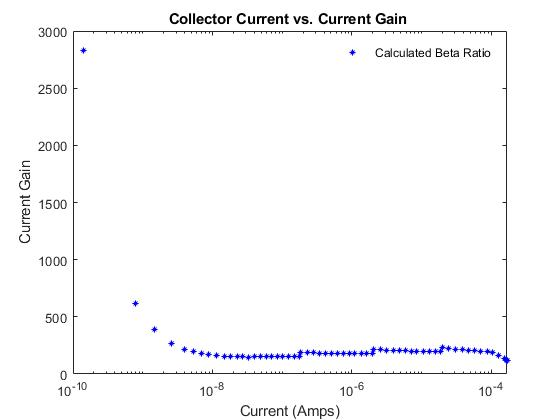
\includegraphics[scale = 0.5]{images/beta_exp1.jpg}
  \caption{The experimental $\beta$ ratio of the transistor.}   
  \label{fig:exp1_beta}
\end{figure}

The logarithmic plot in Figure \ref{fig:exp1_rb} shows the experimental and theoretical incremental base resistance value $r_{b}$ for the bipolar transistor. We calculated experimental incremental resistance with the equation $\frac{\partial V_{in}}{\partial I_{b}}$. 

From our experimental results in Figure \ref{fig:exp1_vc}, we were able to extract values for the thermal voltage, $U_T$. The experimental value for $U_T$ is 0.026 Volts. We used the experimental value of $U_T$ and the value of the base current to calculate and plot the theoretical base resistance in Figure \ref{fig:exp1_rb}.

\begin{figure}[H]   
  \centering        
  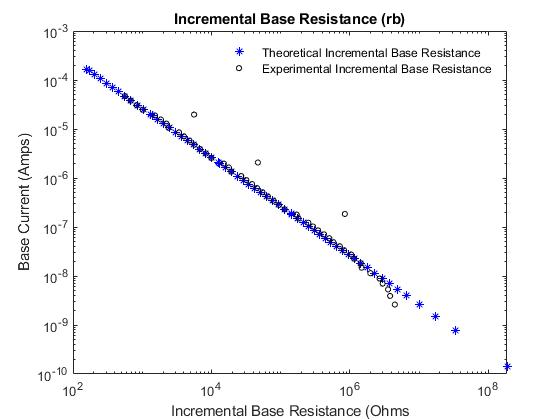
\includegraphics[scale = 0.5]{images/rb_exp1.jpg}
  \caption{The experimental and theoretical incremental base resistance.}   
  \label{fig:exp1_rb}
\end{figure}

The logarithmic plot in Figure \ref{fig:exp1_gm} is a plot of the theoretical and experimental incremental transconductance gain $g_{m}$. Experimental transconductance gain is calculated with $\frac{\partial I_{c} }{\partial V_{in}}$ and the plot shows the base current as a function of transconductance gain.  Using the $U_{T}$ we calculated from the data in Figure \ref{fig:exp1_vc}, we were able to calculate and plot the theoretical transconductance gain.

\begin{figure}[H]   
  \centering        
  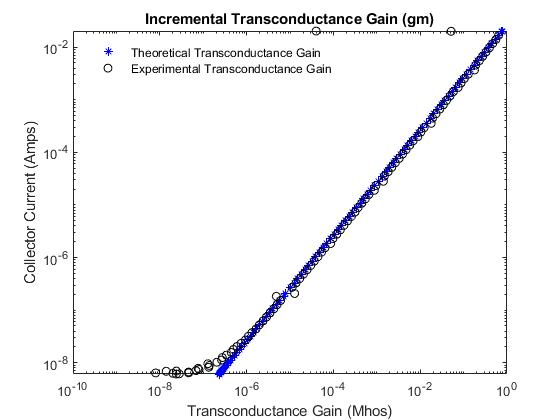
\includegraphics[scale = 0.5]{images/gm_exp1.jpg}
  \caption{The experimental and theoretical incremental transconductance gain.}   
  \label{fig:exp1_gm}
\end{figure}


\subsection{Analysis}
%Plot1
To calculate the collector current that we used in Experiment 1, we rearranged the equation from the pre-lab below to solve for $I_{c}$.
\begin{center}
    $I_{e} =I_{c} + I_{b}$ \\
    $I_{c} = I_{b} - I_{e}$
\end{center} 
To quantify the transistor's resistive behavior, we used the MATLAB $polyfit$ function on the current-voltage characteristic. Specifically, we fit a line to the voltage in at the base and the logarithm of the current output at the collector and at the base. From this linear fit, we could extract the resistance (as the quotient of the voltage and current) in each case. The linear fit had a slope of 37.46 $\Omega$ at the base and a slope of 38.59 $\Omega$ at the collector.

To extract the value of the transistor's thermal voltage, $U_T$, we used linear regression (with the $polyfit$ function in MATLAB) to fit a line to the voltage data points and the logarithm of the current data points from the current-voltage characteristic in Figure \ref{fig:exp1_vc}. We then took the inverse of the determined slope to find the value of $U_T$. The value for $U_{T}$ calculated was 0.026 Volts.

We calculated current gain ($\beta$) by rearranging the equation below from the pre-lab to solve for $\beta$
 \begin{center}
    $I_{b}= \frac{I_{c} }{\beta}$ \\
    $\beta = \frac{I_{c}}{I_{b}}$
 \end{center}
This value, the current gain, is a dimensionless quantity because it refers to the relationship between two current values. 

To calculate the theoretical value of incremental base resistance ($r_b$) for the schematic in Figure \ref{fig:exp1_sch} we used
\begin{center}
    $rb = \frac{U_{T}}{I_{b} }$
\end{center}
from the pre-lab.  To find the experimental value of the incremental base resistance, we used the equation
\begin{center}
    $\frac{\partial V_{in}}{\partial I_{b}}$ 
\end{center}
on the existing current and voltage data. 


To calculate the theoretical value of the incremental transconductance gain ($g_m$) we used 
\begin{center}
    $gm = \frac{I_{c}}{U_{T}}$
\end{center}
from the pre-lab. To find the experimental value of the incremental transconductance gain, we used the equation
\begin{center}
    $\frac{\partial V_{in}}{\partial I_{b}}$ 
\end{center}
on the existing current and voltage data.


\subsection{Discussion}
The collector current follows the exponential relationship with the base voltage.  The range of voltages swept in the lab from .25 to .75 volts highlights the exponential behavior of the relationship between the base voltage and the collector current. This ratio appears linear when plotted on semi-logarithmic axes.

The current gain ($\beta$) follows the trend of exponential decay as current at the collector increases until approximately $10^{-8}$ amps.  When the collector current is greater than $10^{-8}$ amps, the current gain is centered around approximately 180.  $\beta$ is dimensionless because it is  calculated from the ratio of the base current and collector current.

The general slope of the experimental data for the incremental base resistance matches with theoretical expectations.  However, the experimental data does have some clear outliers. To plot the experimental data we took the partial derivative which may have exacerbated any pre-existing anomalies in the collected data.  The general slope of the experimental data for the incremental transconductance gain also aligns with the theoretical model.  However, like in the case of the incremental base resistance, the partial derivative tkaen to calculate $g_{m}$ may have exaggerated any pre-existing anomalies in the collected data.

\section{Experiment Two: Emitter-Degenerated Bipolar Transistor Characteristics}

In Experiment 2, we added a resistor between the emitter of the transistor and ground to make an emitter-degenerated bipolar transistor circuit. The resistor values were $100 \Omega$, $1K \Omega$,  and $10K \Omega$. Figure \ref{fig:exp-2-sch} shows our schematic for this experiment.

\begin{figure}[H] 
  \centering        
  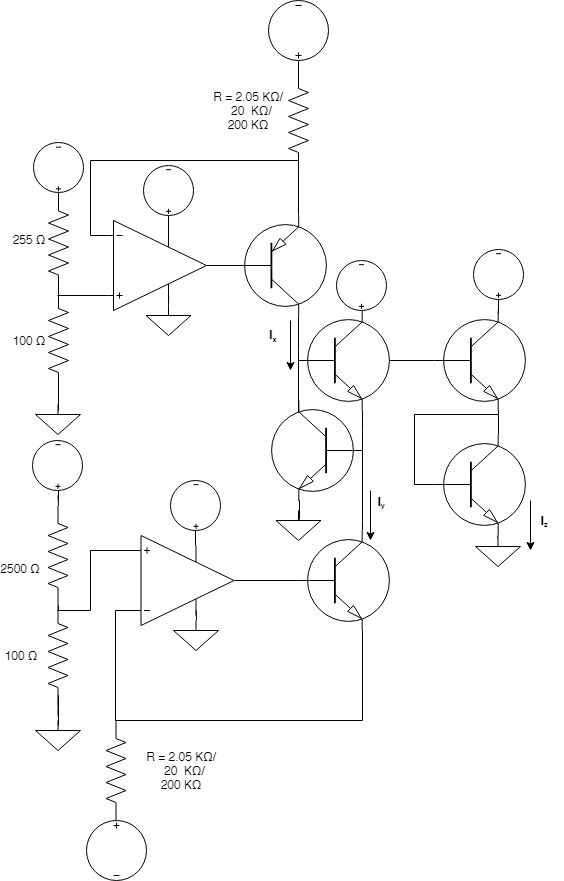
\includegraphics[scale = 0.5]{images/experiment_two_schematic.jpg}
  \caption{Emitter-Degenerated Bipolar Transistor Circuit Schematic.}   
  \label{fig:exp-2-sch}
\end{figure}

\subsection{Results}

In figure \ref{fig:exp2-semilog}, we plotted collector current as a function of base voltage on semi-logarithmic axes for each resistor value.

\begin{figure}[H]   
  \centering        
  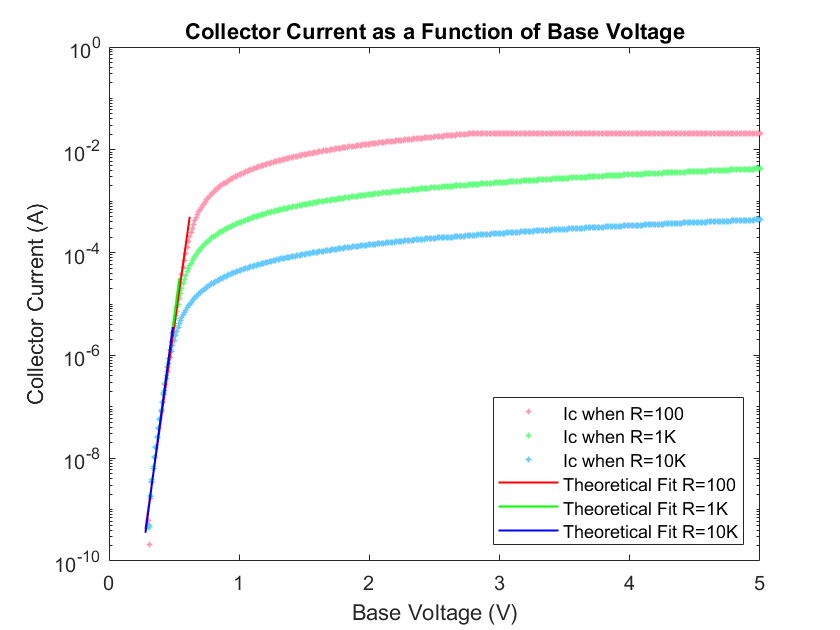
\includegraphics[scale = 0.5]{images/Exp2_Semilog.png}
  \caption{Experimental and Theoretical Base Voltage and Collector Current on semilog axes}   
  \label{fig:exp2-semilog}
\end{figure}

In figure \ref{fig:exp2-linfit-100}, we plotted collector current as a function of base voltage on linear axes with a resistor value of 100 \Omega.

\begin{figure}[H]   
  \centering        
  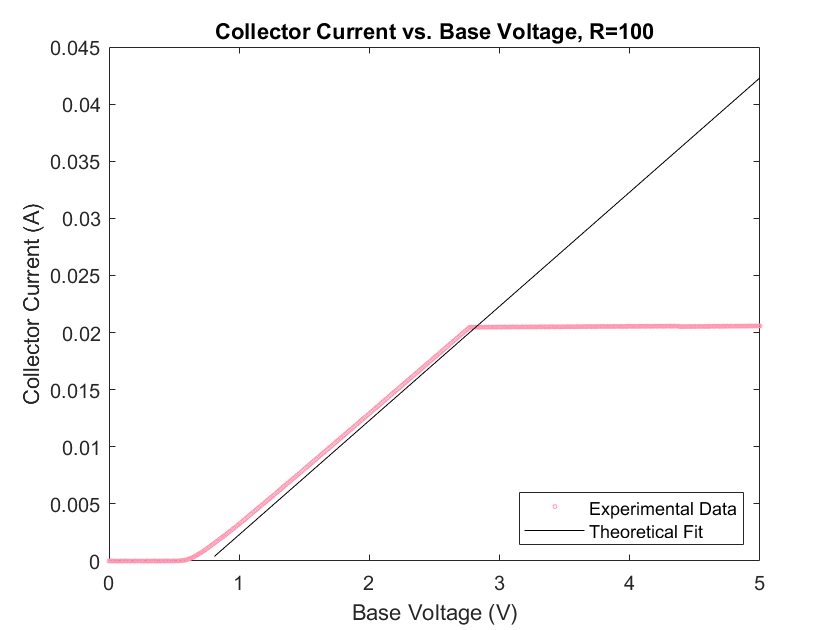
\includegraphics[scale = 0.5]{images/Exp2_LinFit_R100.png}
  \caption{Experimental and Theoretical Base Voltage vs. Collector Current on linear axes with resistor R=100 \Omega}   
  \label{fig:exp2-linfit-100}
\end{figure}

The slope of the current-voltage characteristic when $R=100\Omega$ is $0.0052\frac{A}{V}$
\newline

In figure \ref{fig:exp2-linfit-1K}, we plotted collector current as a function of base voltage on linear axes with a resistor value of 1K\Omega.

\begin{figure}[H]   
  \centering        
  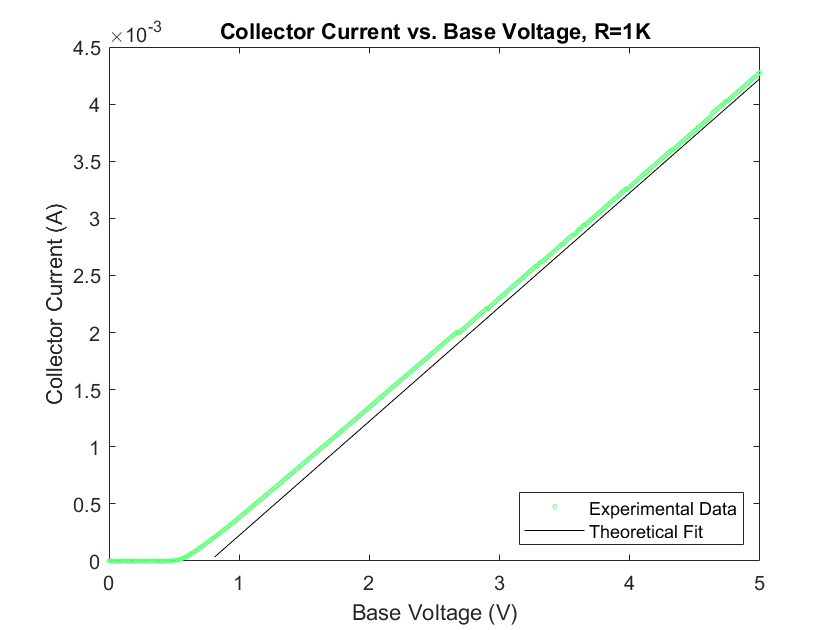
\includegraphics[scale = 0.5]{images/Exp2_LinFit_R1K.png}
  \caption{Experimental and Theoretical Base Voltage vs. Collector Current on linear axes with resistor R=1K \Omega}   
  \label{fig:exp2-linfit-1K}
\end{figure}

The slope of the current-voltage characteristic when $R=1K\Omega$ is $9.2788 x 10^{-4}\frac{A}{V}$
\newline

In figure \ref{fig:exp2-linfit-10K}, we plotted collector current as a function of base voltage on linear axes with a resistor value of 10K \Omega.

\begin{figure}[H]   
  \centering        
  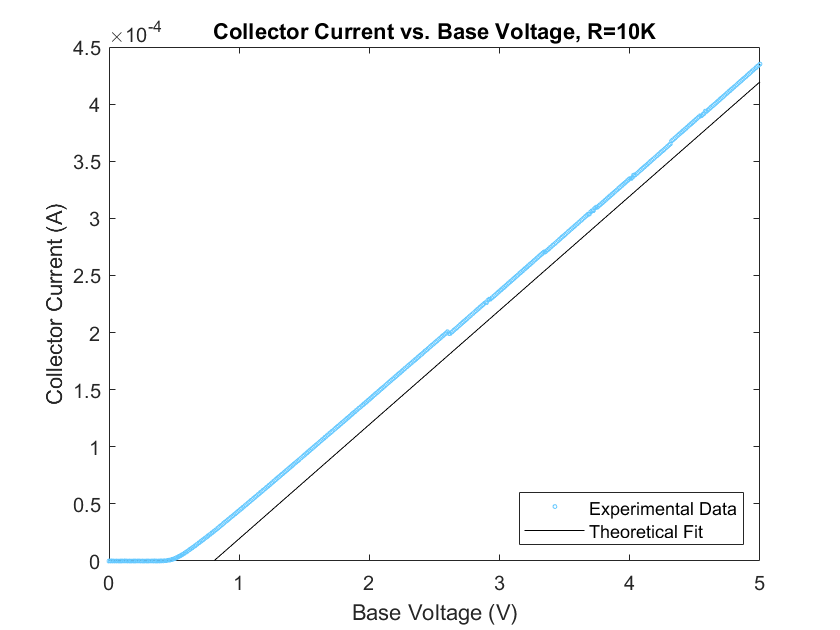
\includegraphics[scale = 0.5]{images/Exp2_LinFit_R10K.png}
  \caption{Experimental and Theoretical Base Voltage vs. Collector Current on linear axes with resistor R=10K \Omega}   
  \label{fig:exp2-linfit-10K}
\end{figure}

The slope of the current-voltage characteristic when $R=1K\Omega$ is $9.3737 x 10^{-5}\frac{A}{V}$
\newline

In figure \ref{fig:exp2-rb} we plotted incremental base resistance as a function of base current for the transistor in series with each resistor. 

\begin{figure}[H]   
  \centering        
  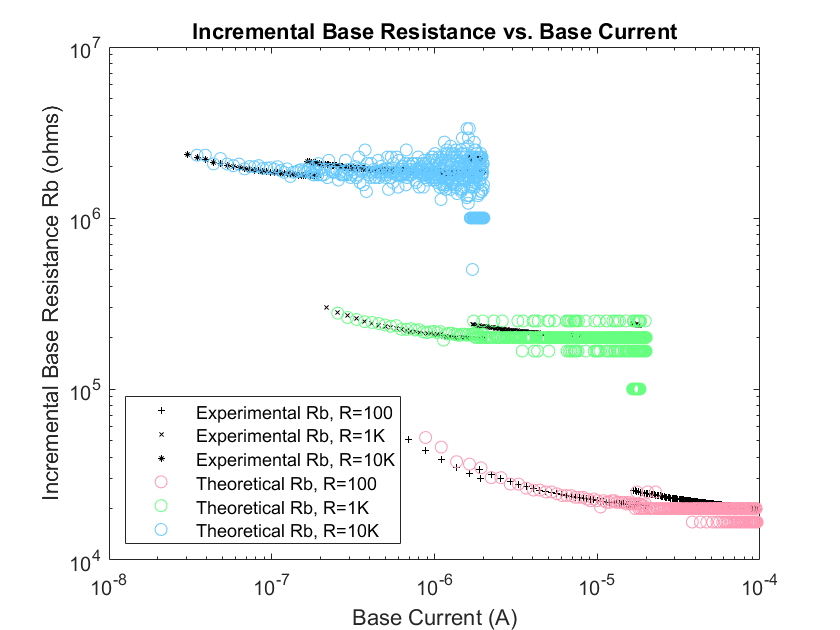
\includegraphics[scale = 0.5]{images/Exp2_rb.png}
  \caption{Experimental and Theoretical Incremental Resistance as a function of Base Current}   
  \label{fig:exp2-rb}
\end{figure}

In figure \ref{fig:exp2-gm} we plotted incremental transconductance gain  for the transistor in series with each resistor value as a function of collector current.

\begin{figure}[H]   
  \centering        
  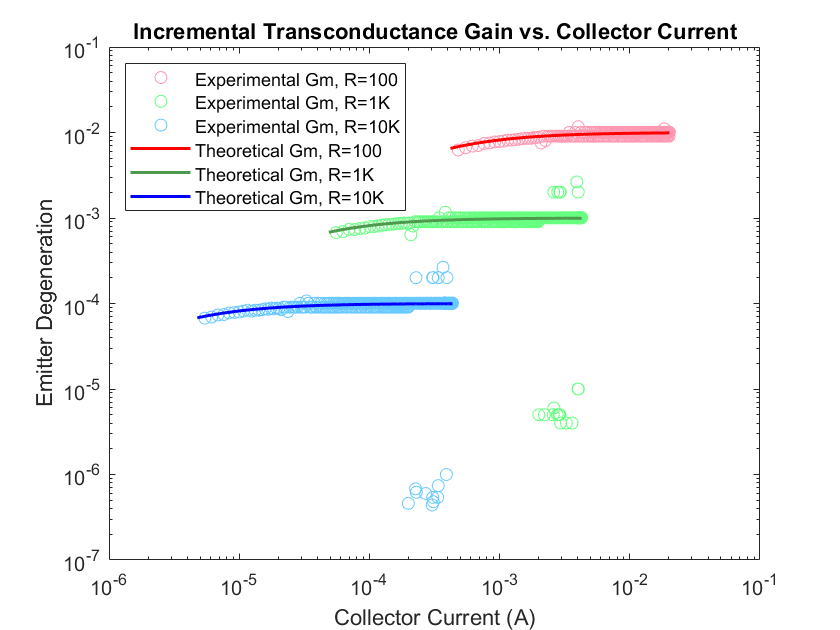
\includegraphics[scale = 0.5]{images/Exp2_gm.png}
  \caption{Experimental and Theoretical incremental transconductance gain as a function of collector current}   
  \label{fig:exp2-gm}
\end{figure}

\subsection{Analysis}
Since instrumentation constraints prevent direct measurement of collector current, we instead measured the emitter and base currents and then calculated collector current from our data using the equation

\begin{centering}
    $$I_c = I_e - I_b$$
\end{centering}

For the theoretical current-voltage fits for the semilog and linear axes plots in figures \ref{fig:exp2-semilog} - \ref{fig:exp2-linfit-10K}, we calculated the distinct regions of behavior, before and after the $V_{on}$ voltage, with different equations.
We extracted $U_t$ and $I_s$ from the inverse of the slope and exponential of the intercept of a $polyfit$ of the linear part of the semilog plotted current-voltage characteristic.

Since the transistor is the dominant component in the circuit when $V_{in}$ is less than $V_{on}$, we can use the following equation to model the collector current.

\begin{centering}
$$I_c = I_s  e^{\frac{V_{b}}{U_t}}$$ 
\end{centering}

Since this section of the theoretical fit is exponential, it appears linear on the semilog axes in figure \ref{fig:exp2-semilog}. We plotted the experimental data on semilog axes (the y axis is logarithmic).

When $V_{in}$ is greater than $V_{on}$, we used the following equation to calculate the theoretical fit to reflect that the  resistor dictates this region of the circuit's behavior.

\begin{centering}
$$I_c = \frac{V_b - V_{on}}{R}$$
\end{centering}

In this section of the current-voltage fit it appears to be linear, so we plotted this theoretical fit on linear axes in figures \ref{fig:exp2-linfit-100}, \ref{fig:exp2-linfit-1K}, \ref{fig:exp2-linfit-10K}. We also plotted all the experimental data on linear axes for these figures. 

In the linear axes plots, there are small offsets between the experimental and theoretical lines, but the slopes are very similar. 

For figure \ref{fig:exp2-rb}, we calculated the theoretical fit for the incremental resistance using this equation from the prelab.

\begin{centering}
$$R_b = \beta R (1 + \frac{I_{on}}{\beta I_b)}$$
\end{centering}

Since $\beta$ is equal to $\frac{I_c}{I_b}$ and $I_{on}$ is equal to $\frac{U_t}{R}$, we can re-write this equation as

\begin{centering}
$$R_b = \frac{U_t}{I_b} + \frac{I_c}{I_b}R$$
\end{centering}

To plot the experimental data for $R_b$, we took the derivative of $V_b$ over $I_b$ based on the equation derived in the packet

\begin{centering}
$$R_b = \frac{\delta V_b}{\delta I_b}$$
\end{centering}

In MATLAB, we used the $diff$ function to take these partial derivatives. 
There are some outliers in the experimental points on the plot, perhaps due to a discontinuity in the data that became more apparent when we took the partial derivatives. 

\newline

For figure \ref{fig:exp2-gm}, we calculated the incremental transconductance gain using this equation from the prelab

\begin{centering}
$$G_m = \frac{1}{R} \cdot \frac{1}{1 + U_t / I_c R}$$
\end{centering}

To calculate the experimental incremental transconductance gain, we used this equation from the packet

\begin{centering}
$$G_m = \frac{\delta I_c}{\delta V_b}$$
\end{centering}

There are some outliers in the experimental points on the plot, which is again perhaps due to a discontinuity in the data that became more apparent when we took the partial derivatives. 


\subsection{Discussion}
Although the transistor is not diode connected (as it was in Lab 2), we still see two qualitatively distinct regions of operation. Overall, the theoretical fits and measured component behaviors align fairly well; the experimental behavior conforms to mathematical expectations, and we can reasonable characterize emitter-degenerated bipolar transistor configuration. A few exceptions where our predictions did not match the data include large outliers in the incremental base resistance and transconductance gain plots and a notable offset between the theoretical and experimental collector current. 

For each resistor value, we found that the slope of the lineear portion of the semi-logarithmic current-voltage characteristic remained constant. However, the base voltage at which the current response diverged from exponential behavior and instead became nearly constant changed by resistor value; specifically, there is a direct inverse relationship between the resistor value and the value at which the current becomes constant - as we increased the resistor value by an order of magnitude, the current at which the current-voltage characteristic became nearly constant decreased by an order of magnitude.

\section{Experiment Three : Voltage Emitter-Follower}
In experiment three, we built an emitter-follower circuit. More specifically, we constructed a common-collector amplifier, where the collector is kept at a standard potential, voltage input occurs at the base, and voltage output measurement occurs between the emitter and a resistor connected to ground.
\begin{figure}[H]   
  \centering        
  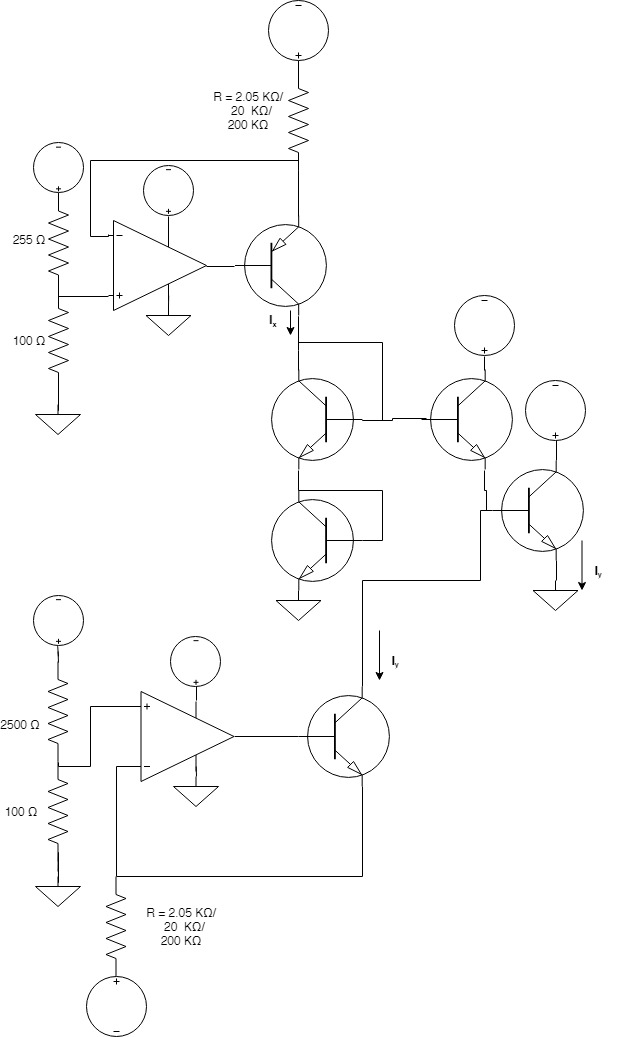
\includegraphics[scale =0.5] {images/experiment_three_schematic.jpg}
  \caption{Experiment Three Emitter-Follower Schematic.}
  \label{fig:schem3}
\end{figure}
\subsection{Results}
This plot shows the emitter-follower's experimental voltage transfer characteristic (the response of V$_{out}$ depending on changes in V$_{in}$) and a theoretical fit.
\begin{figure}[H]   
  \centering        
  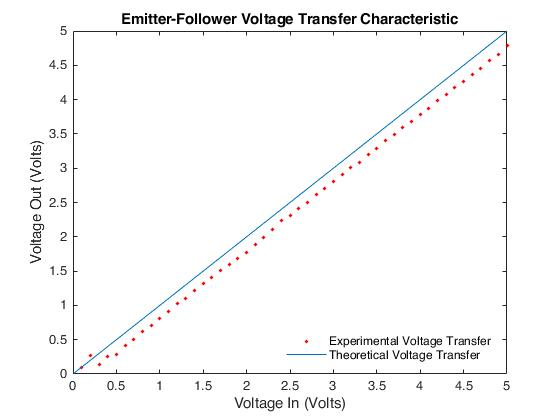
\includegraphics[scale =0.5] {images/experiment_three_plot.jpg}
  \caption{Emitter-Follower Voltage Transfer Characteristic.}
  \label{fig:plot3}
\end{figure}
Using MATLAB's $polyfit$ finction, we found that the slope of the line formed by the points in the experimental data is $.9779$. This ratio is dimensionless.

\subsection{Analysis}
An emitter-follower circuit should create a direct voltage buffer between the input and output; ideally, as the base voltage increases, the emitter voltage also increases by the same proportion.  Therefore, the slope of the voltage transfer characteristic should be $1$. Because this is a ratio between voltages, this slope has no units attached to its value. The x-intercept and y-intercept of this line should be equal to the turn-on voltage of the transistor in this particular configuration.

To create the voltage transfer  characteristic, we swept the base voltage from 0 Volts to 5 Volts. We then used MATLAB's  $polyfit$ function on the sampled data and determined that the  experimental ratio between the input voltage and the output voltage was $.9779$. The experimental voltage is consistently lower than the ideal voltage. 

The amount of error between the ideal and experimental slope (which is a dimensionless quantity) is $\frac{(1 - .9779)}{1} = .0221$, or $2.21\%$.  

\subsection{Discussion}
The ideal incremental voltage gain of the emitter follower is equal to $1$ because the input voltage at the base should follow directly to the output voltage at the emitter. In the experimental case, the incremental voltage gain is equal to $.9779$, so the voltage out is equal to $.9779$ times the voltage in. On average, the experimental voltage output is $.23$ Volts less than the voltage input for each point - this difference is associated with the voltage drop across the transistor's base-emitter junction and the voltage divider created by the 100 $\Omega$ resistor following the transistor and is approximately equal to the turn-on voltage of the given transistor. This value is slightly lower than the expected turn-on voltage, which is likely due to the offset associated with the resistor value and the base-emitter voltage difference of the transistor itself.
% TODO try to come up with a better explanation here...

\section{Experiment Four : Inverter}
In experiment four, we created a common-emitter amplifier circuit by adding a resistor to the voltage follower circuit in between the collector voltage source and the collector. The value of the resistor at the collector is some integer multiple of the resistor at the emitter.

\begin{figure}[H]   
  \centering        
  \includegraphics[scale =0.5] {images/experiment_four_schematic.jpg}
  \caption{Schematic of the inverter/common emitter-amplifier circuit.}
  \label{fig:schem_4}
\end{figure}

\subsection{Results}
The plot below shows the emitter-amplifier circuit's voltage transfer characteristic for three separate collector resistor values. 
\begin{figure}[H]   
  \centering        
  \includegraphics[scale =0.3] {images/experiment_four_plot.jpg}
  \caption{Voltage transfer characteristic of the inverter circuit.}
  \label{fig:plot_4}
\end{figure}
\subsection{Analysis}
The theoretical value of the voltage transfer relationship between the base and collector can be illustrated by two distinct regions of operation. Once the input voltage has exceeded the base-emitter voltage difference (approximately .65 Volts), the transistor is in forward active mode. Then, the voltage output at the collector relative to the base voltage decreases linearly by means of Ohm's Law, where the $V_{out}$ is equal to the $V_{collector} - I_{collector}R_{collector}$. 
Eventually, as $V_{collector}$ decreases and $V_{base}$ increases, the transistor enters saturation mode; the value of the voltage output instead roughly equals the voltage input offset by the original .65 Volts. Then, this line then becomes symmetrical with the original emitter-follower response. More rigorously, the incremental voltage gain for each circuit should be equal to $-m$, and the turn-around point should be associated with when the voltage into the base of the transistor is greater than the collector voltage when offset by the resistor. We can calculate this value using $\frac{(V_{collector} + mV_{on})}{m+1}$, where $m$ is the integer quotient between the collector resistor value and the emitter resistor value.  . In the case of the 200 $\Omega$ resistor, this would result in a slope of -2 for the original inversion, and a turn-around point of 2.30 Volts. For the 300 $\Omega$ resistor, this would be a slope of -3 and a turn-around point of 2.0 Volts. For the 400 $\Omega$ resistor, this would result in a slope of -4 and a turn-around point of 1.75 Volts.

Experimentally, the transistor showed a change to forward active mode at .65 Volts. This shift changed the slope of the incremental voltage gain based on the quotient of the collector and emitter resistance values. To calculate the experimental incremental voltage gain, we used MATLAB's $polyfit$ function on the portion of voltage outputs associated with voltage inputs greater than the base-emitter voltage and less than the turn-around current, which we calculated using the equation $\frac{(V_{collector} + mV_{on})}{m+1}$, where $m$ is the integer quotient between the collector resistor value and the emitter resistor value.  

The 200 $\Omega$ resistor yielded an inverted incremental voltage gain of approximately 1.89 and it had a turn-around point of approximate 2.35 Volts, the 300 $\Omega$ resistor yielded an incremental voltage gain of approximately 2.80 and a turn-around voltage of 1.94 Volts, and the 400 $\Omega$ resistor yielded an inverted incremental voltage gain of approximately 3.73 and a turn-around voltage of 1.69 Volts. Note that the value of the voltage gain should be dimensionless.

For the 200 $\Omega$ resistor, the error for the slope was $\frac{2-1.89}{2}$ = $.055$, or $5.5\%$. The error for the turn-around point was $\frac{2.35 Volts -2.30 Volts}{2.35 Volts}$ = $.021$, or $2.1\%$. For the 300 $\Omega$ resistor, the error for the slope was $\frac{3-2.80}{3}$ = $.067$, or $6.7\%$. The error for the turn-around point was $\frac{2.0 Volts -1.94 Volts}{2.0 Volts}$ = $.03$, or $3\%$. For the 400 $\Omega$ resistor, the error for the slope was $\frac{4-3.73}{4}$ = $.068$, or $6.8\%$. The error for the turn-around point was $\frac{1.75 Volts - 1.69 Volts}{1.75 Volts }$ = $.034$, or $3.4\%$. 

\subsection{Discussion}

For each collector resistor, in the voltage range where the transistor is in forward active mode, the incremental voltage gain of the resistor is nominally equal to $-m$, or the negative integer quotient of the collector resistor and the emitter resistor. Because our emitter resistor was 100 $\Omega$, when our collector resistor was 200 $\Omega$, are incremental voltage gain was approximately 2; when the resistance was 300 $\Omega$, the gain was approximately 3, and when the resistance was 400 $\Omega$, the gain was approximately 4. The reason that this relationship is  direct is because the collector resistor and emitter resistor invert and increase the resulting collector voltage prior to the drop across the transistor. This continues until the input voltage exceeds this output voltage, and then the transistor enters saturation mode and displays behavior that matches that of the emitter-follower.

For each slope and turn-around point, there was a small discrepancy between the theoretical and empirical data points. The reason that this occurred is because when the voltage difference between the collector and base is within a few $U_T$, the transistor is in soft saturation mode (and so it curves instead of directly transitioning to displaying emitter-follower behavior) and it has existing current that slows the transitional behavior. For that reason, both the empirical slopes and the empirical turn-around points are slightly lower than the theoretical ones.  


\end{document}
